\section{External Interface Requirement}
\subsection{User Interfaces}

\begin{figure}[ht]
    \centering
    \begin{subfigure}[t]{0.38\linewidth}
        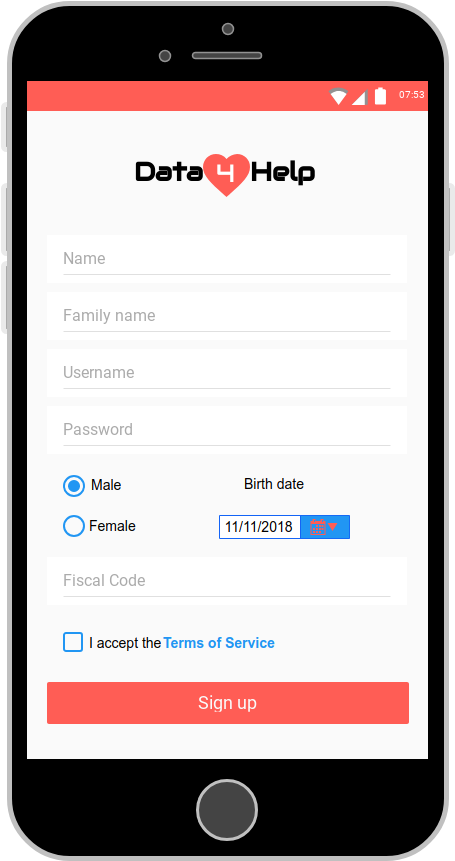
\includegraphics[width=\linewidth]{images/Mock-up/Sign_Up_Page.png}
        \caption{Data4Help Sign Up.}
    \end{subfigure} \hfil \hfil \hfil
    \begin{subfigure}[t]{0.38\linewidth}
        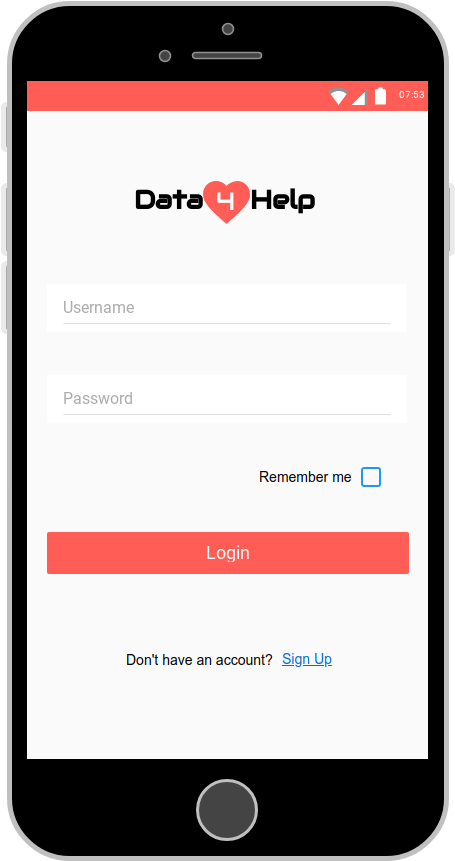
\includegraphics[width=\linewidth]{images/Mock-up/Login_Page.png}
        \caption{Data4Help Login.}
    \end{subfigure}
\end{figure}

\begin{figure}[ht]
  \centering
  \begin{subfigure}[t]{0.38\linewidth}
    \addtocounter{subfigure}{2}
    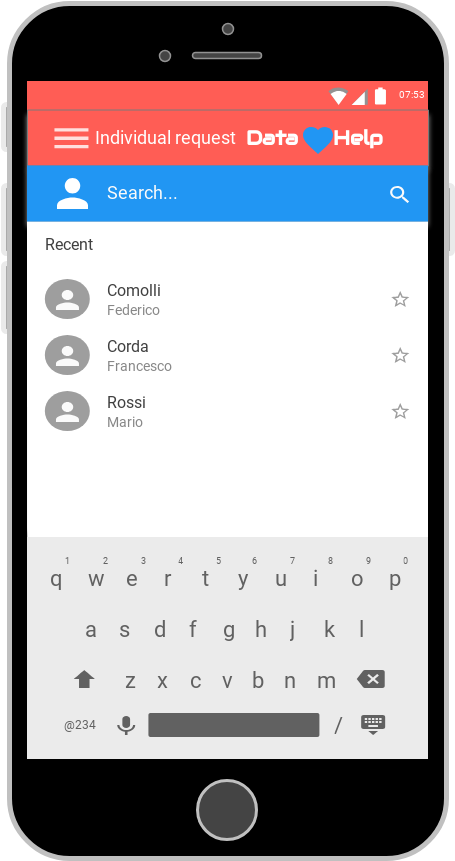
\includegraphics[width=\linewidth]{images/Mock-up/Individual_Request_1.png}
    \caption{TP researches a user.}
  \end{subfigure} \hfil \hfil \hfil
  \begin{subfigure}[t]{0.38\linewidth}
    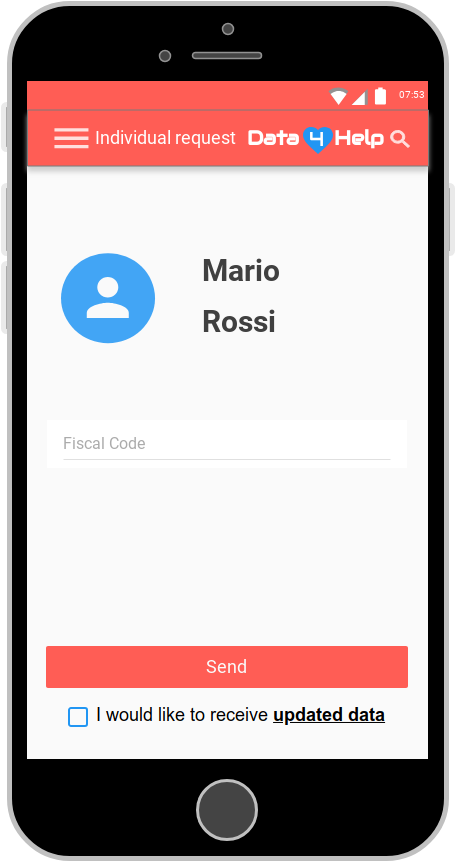
\includegraphics[width=\linewidth]{images/Mock-up/Individual_Request_2.png}
    \caption{TP inserts a user's Fiscal Code.}
  \end{subfigure}
\end{figure}

\begin{figure}[ht]
  \centering
  \begin{subfigure}[t]{0.38\linewidth}
    \addtocounter{subfigure}{4}
    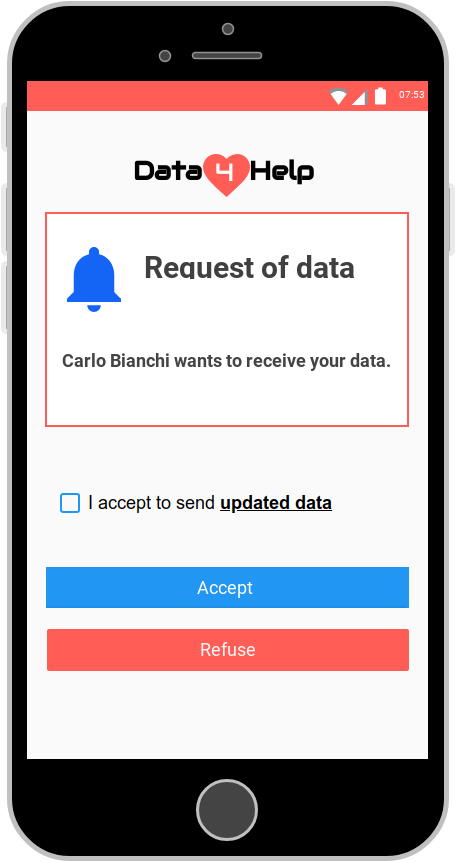
\includegraphics[width=\linewidth]{images/Mock-up/Acceptdecline_request.png}
    \caption{User accepts a request.}
  \end{subfigure} \hfil \hfil \hfil
  \begin{subfigure}[t]{0.38\linewidth}
    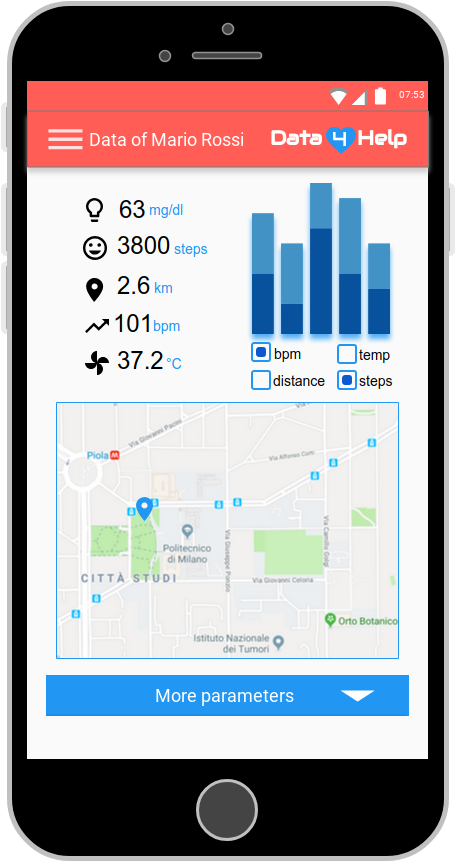
\includegraphics[width=\linewidth]{images/Mock-up/IndividualDataTP.png}
    \caption{TP accesses to data of a user.}
  \end{subfigure}
  %\caption{***}
  %\label{fig:images}
\end{figure}

\begin{figure}[ht]
  \centering
  \begin{subfigure}[ht]{0.38\linewidth}
    \addtocounter{subfigure}{6}  
    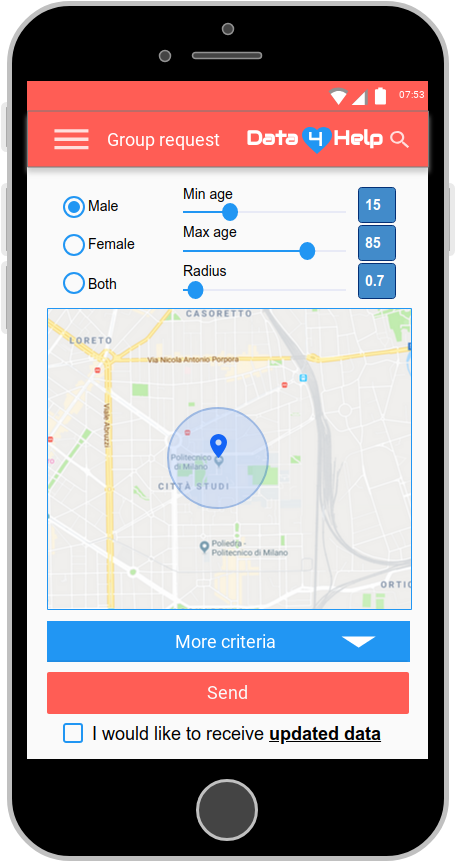
\includegraphics[width=\linewidth]{images/Mock-up/Group_Request.png}
    \caption{TP creates a group request.}
  \end{subfigure} \hfil \hfil \hfil
  \begin{subfigure}[ht]{0.38\linewidth}
    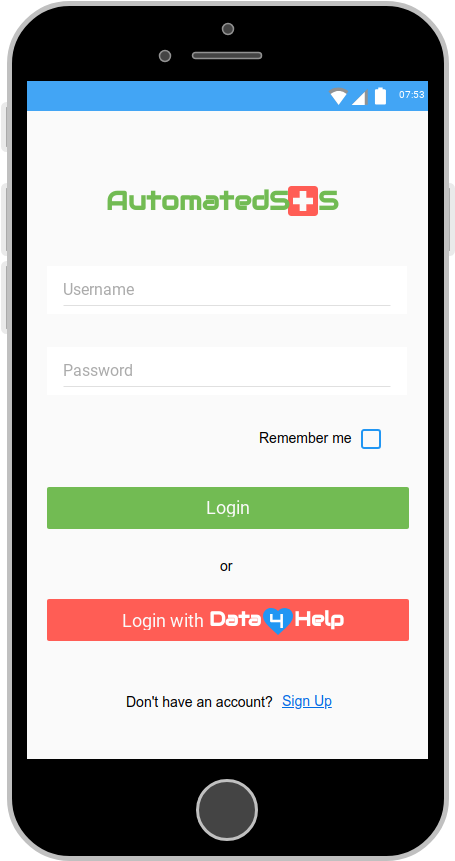
\includegraphics[width=\linewidth]{images/Mock-up/AutomatedSOS_Login.png}
    \caption{AutomatedSOS Login.}
  \end{subfigure}
  %\caption{***}
  %\label{fig:images}
\end{figure}

\begin{figure}[ht]
  \centering
  \begin{subfigure}[ht]{0.38\linewidth}
    \addtocounter{subfigure}{8}  
    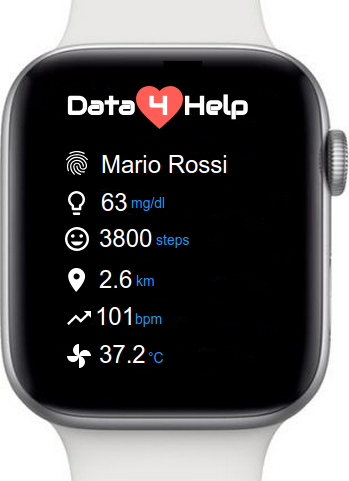
\includegraphics[width=\linewidth]{images/Mock-up/Wearable.png}
    \caption{User accesses to his/her own data.}
  \end{subfigure} \hfil \hfil \hfil
  \begin{subfigure}[ht]{0.38\linewidth}
    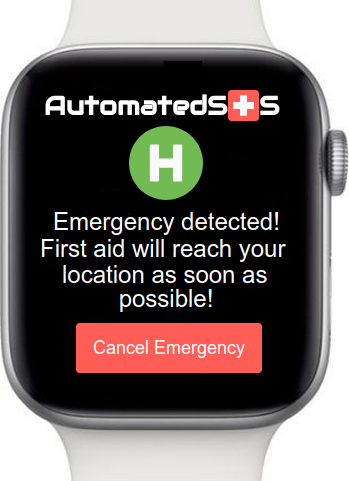
\includegraphics[width=\linewidth]{images/Mock-up/Wearable_2.png}
    \caption{User receives the First Aid notification.}
  \end{subfigure}
  %\caption{***}
  %\label{fig:images}
\end{figure}

\begin{figure}[ht]
    \renewcommand{\thefigure}{\alph{figure}}
    \centering
    \addtocounter{figure}{5}
    \captionsetup{labelformat=parens, labelsep=space, name=}
    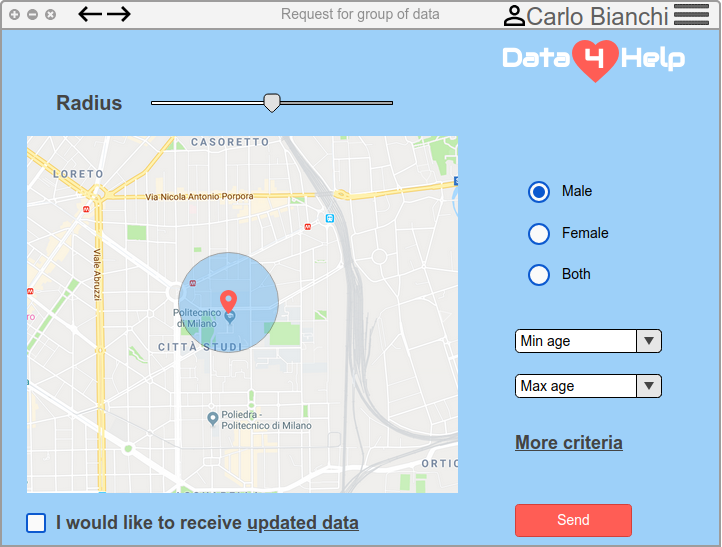
\includegraphics[width=300pt]{images/Mock-up/Third_Party_req_WP.png}
    \caption{TP creates a group request.}
\end{figure}

\begin{figure}[ht]
    \renewcommand{\thefigure}{\alph{figure}}
    \centering
    \captionsetup{labelformat=parens, labelsep=space, name=}
    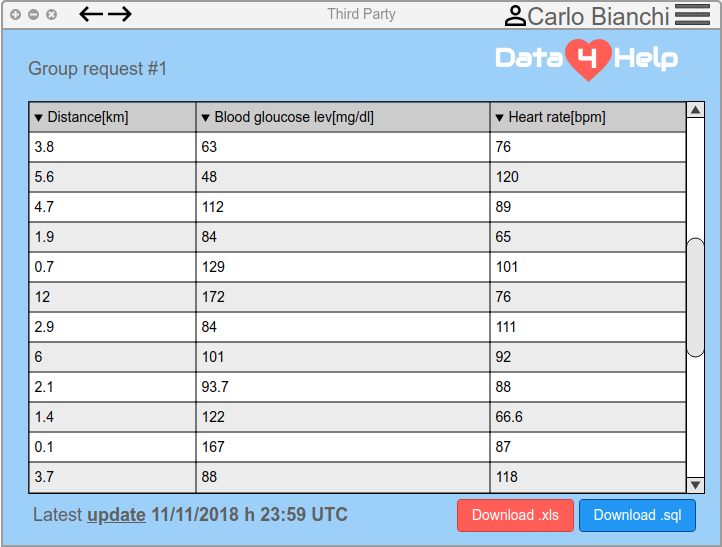
\includegraphics[width=300pt]{images/Mock-up/Third_Party_webPage.png}
    \caption{TP accesses to an anonymized group of data.}
\end{figure}
\clearpage

\subsection{Hardware Interfaces}
Data4Help and AutomatedSOS are not designed to offer hardware interfaces to interact with external services.
\subsection{Software Interfaces}
Data4Help will offer an API to let third parties access to users' data.
\subsection{Communication Interfaces}
The system will perform its communications using the HTTPS and TCP/IP protocols.

\section{Scenarios}
    \subsection{Scenario 1}
    Nike is a worldwide brand of sportswear mainly focused on shoes. The company wants to introduce a new model of shoes addressed to younger people that live in metropolis. Carl, the research manager of the company, wants to understand the habits concerning walking of the young people who are the target for this new model of shoes.
    Fortunately, he has just read on a famous daily newspaper about a new service called Data4Help, which collects data of a huge amount of people all around the world. \\
    After Carl has been registered to the service, he can make a request for data by filling the apposite form. Data4Help offers the possibility to customize a request by selecting a range for some categories. He selects as parameters of the request \say{people living in city with more than one million inhabitants} and \say{people aged between 15 and 25 years}. \\
    TrackMe approves the request since it refers to more than 1000 people and it sends to Carl all the demanded data.
    Now Carl can carry on his project since he know the target's habits.

    \subsection{Scenario 2}
    Anna is really worried since her mother's latest accident. Her mother is elderly and from now on, also due to the broken foot, has to rest to bed for some period. Martha, a friend of Anna, recommends her a new system of monitoring health status focused on elderly people. \\ 
    After a short research on the net, she downloads AutomatedSOS on her mobile phone and buys a specific electronic device compatible with the app to be supplied to her mother. 
    Anna registers her mother to the service by filling the gaps (username, password and Fiscal Code) in the interface provided by AutomatedSOS.
    After the confirmation message, it starts to acquire health parameters (such as position, heart rate, skin temperature, blood glucose level and so on) and it sends them to AutomatedSOS every 2 seconds.
    Anna can breathe a sigh of relief: whenever her mother will be in danger, AutomatedSOS will detect it by comparing the parameters provided by the electronic device with specific thresholds. \\ 
    If an emergency occurs, AutomatedSOS will send a request to the Operations Center of the NHS for an ambulance within 5 seconds. The request will include the parameters and her position, so that the ambulance can estimate the alert level, it can reach Anna’s mother and can provide her first aid. \\
    Hope it will never occur!

    \subsection{Scenario 3}
    Bianca is very caring for her son Mark, a 15 years old teenager very lively.
    Mark’s passion is the bike and, unfortunately, he has no friends with whom he could share this sport. At least twice a week Mark, after school, takes a bike ride with his mountain-bike both for the roads and for the wood.
    He is always alone while he is riding so Bianca is worried about Mark safeness.
    Bianca’s hair stylist tell her about a system that monitor real-time position of its users. \\
    She obliges Mark to download and register to Data4Help application on his smart phone and, meanwhile, also Bianca does it.
    After the login, Bianca makes a request for Mark position by inserting in the apposite form his Fiscal Code. She also subscribes to receive the updated position as soon it is available. \\
    Mark has only to accept the request of Bianca by pressing the specific button in the Data4Help interface and doing so, he can riding careless of his mother...she always knows his position and she is more quiet. At most every 2 seconds, the GPS on Mark’s smart phone collects and sends the latest position to Data4Help system. Once the system receives a new position, it forwards it within 2 seconds to Bianca’s smart-phone. Bianca now can find Mark’s actual position by looking it into the Data4Help interface.
    Well done!
    
    \subsection{Scenario 4}
    Clara's life is a bit difficult since she was diagnosed with diabetes 5 years ago.
    Up to now she used the traditional method consisting of a blood injection three times a day, every day, to monitor her glucose level.
    During her last periodical check, the doctor told her about a new smart-watch for monitoring blood glucose level in a non intrusive way, detecting it through the sweat. \\
    This smart-watch is equipped with Data4Help, an innovative system able to collect health parameters of the users.
    Clara must simply download Data4Help app and register with her personal information (name, surname, age, gender, Fiscal Code or SSN). \\
    Clara life is simpler from now on, she has just to look the parameters on her smart-watch to know in real time her health status.
    Another functionality of Data4Help allows Clara's doctor to monitor in real-time her patient. After registering to Data4Help as a third party, the doctor makes a request for individual data inserting Clara's name, surname and Fiscal Code. In order to receive a continuum stream of data, the doctor makes a subscription request to Clara's parameters.
    Clara has to accept these requests through the functionality provided by Data4Help.
    The doctor has all Clara's parameters in real time and can monitor her health status.
    Next check up will be much faster.
    
    \subsection{Scenario 5}
    Tom is an avid smoker from many years and suffers of respiratory problems. For this reason he often goes to the doctor to monitor his lungs status.
    Tom's last visit showed a critical health status, so his doctor prescribed him to download AutomatedSOS app on his smart-watch.
    Tom must register to AutomatedSOS by inserting his credentials (name, surname, age, gender, Fiscal Code or SSN) in order to be monitored in real-time. \\
    AutomatedSOS is built on top of Data4Help, a service that acquires position and health parameters of its users and makes them available to third parties.
    Tom's doctor uses Data4Help to monitor his patient's health status by requesting a subscription to his parameters through the apposite function.
    Tom can accept the request using AutomatedSOS app, since it includes all the Data4Help's functionalities. \\
    One day, while he is on his way to work, he starts not feeling good. AutomatedSOS system detects an anomaly in the parameters and immediately finds out that that an emergency is occuring. 
    Within 5 seconds from the moment that parameters are received, the system sends a request to the OC of the NHS. \\
    The request includes Tom health parameters and his position so that NHS can estimates the alert level and provide him first aid.
    As soon as the request arrives at the OC, the situation is clear: Tom is having an heart attack. An ambulance is promptly sent to Tom's location and it arrives within 10 minutes from the moment of the illness.
    Few minutes more would have been fatal. \\
    Great job AutomatedSOS!
    
    \subsection{Scenario 6}
    Oliver is the responsible of a sports center which includes also an athletic track.
    At the moment the track is not in the best condition, since it was built 10 years ago, when the sports center opened.
    Oliver would like to restore the track but he wants to be sure that his costumers use it frequently and that the average of the training's length is more than 5 km. \\
    Oliver is already a user of Data4Help and knows all the functionalities provided by that service. He asks to all the customers of the sports center that use the athletic track to download and register to Data4Help application on their devices. If they don't own one, Oliver would provide them with a smart-watch. \\
    Of course, during the whole training the customers must bring with them a device equipped with Data4Help and the GPS.
    Now Oliver has just to make a request to access to data of a group of people. \\
    Through the functionality provided by the app, Oliver fills the form by selecting the following criteria: \say{People that do physical activities from 8 AM to 10 PM} (the opening hours of the sports center) and \say{People that do physical activities within 1 km far for Elizabeth road, London, UK} (the location of the sports center).
    Unfortunately, only 438 people corresponds to those criteria so the system denies the request made by Oliver.
    A negative message appears on his smart-phone showing the reason for the declined data.
    Oliver has to find a new way to discover if the investment is a good idea. \\
    Try again, you'll be luckier.

\section{Functional Requirements}
\textbf{Data4Help:}  
\begin{enumerate} [label={\bf[G\arabic*]}]
    \item \textbf{Allow a visitor to become registered user after providing credentials.}
        \begin{itemize}
            \item [{[D1]}] Users insert credentials that correspond to their identity.
            \item [{[D2]}] When a new registered user sends his/her credentials to the system, the message will be surely received.
            \item [{[R1]}] The system should provide a registration form offering the following mandatory fields: name, surname, SSN or Fiscal Code.
            \item [{[R2]}] The system must guarantee that the credentials are unique.
        \end{itemize}
        
    \item \textbf{Monitor the location of users through electronic devices.}
        \begin{itemize}
            \item [{[D3]}] The communication channel doesn't corrupt the data sent by the user's device to the system and vice versa.
            \item [{[D4]}] The electronic device on which the system is installed is equipped with the GPS sensor.
            \item [{[D6]}] The  system  retrieves  the  data  from  the  sensors through the interfaces available on the electronic device.
            \item [{[D7]}] Position information provided by GPS is sufficiently accurate.
            \item [{[R3]}] The system must acquire real-time users' positions from the GPS installed on the user's device.
            \item [{[R4]}] The system must collect users' data in specific databases.
        \end{itemize}
        
    \item \textbf{Monitor the health status of users through electronic devices.}
        \begin{itemize}
            \item [{[D3]}] The communication channel doesn't corrupt the data sent by the user's device to the system and vice versa.
            \item [{[D5]}] The electronic device on which the system is installed is equipped with the sensors related to the parameters tracked by Data4Help.
            \item [{[D6]}] The  system  retrieves  the  data  from  the  sensors  through  the  interfaces available on the electronic device.
            \item [{[D8]}] The sensors related to the health status collect the data with a reasonable precision.
            \item [{[R5]}] The system must acquire real-time users' health parameters from the sensors installed on the user's device.
            \item [{[R4]}] The system must collect users' data in specific databases.
        \end{itemize}
        
    \item \textbf{Allow a user to accept or refuse a request to access to personal data.}
    \begin{itemize}
            \item [{[R6]}] Every time that a third party inserts a request for data relative to a Fiscal Code, the system must ask the authorization to the corresponding user.
            \item [{[R7]}] The system must provide a function to allow users to accept or refuse a request for personal data.
        \end{itemize}

    \item \textbf{Allow third parties to register to the system.}
        \begin{itemize}
            \item [{[D1]}] Users insert credentials that correspond to their identity.
            \item [{[D1]}] When a new registered user sends his/her credentials to the system, the message will be surely received.
            \item [{[R8]}] The system should provide a registration form to third parties.
            \item [{[R2]}] The system must guarantee that the credentials are unique.
        \end{itemize}
        
    \item \textbf{Allow third parties to request an access to users' data.}
    \begin{enumerate} [label*={.\arabic*}]
        \item [\bf{[G6.1]}] \textbf{Allow third parties to request access to data of some specific individuals by providing SSN or Fiscal Code.}
            \begin{itemize}
                \item [{[R9]}] The system must provide a function to allow third parties to request the access to individuals data. The form must require the filling of the SSN or Fiscal Code of the corresponding user.
            \end{itemize}
        \item [\bf{[G6.2]}] \textbf{Allow third parties to request access to anonymized data of group of people.}
            \begin{itemize}
                \item [{[R10]}] The system must provide a function to allow third parties to request the access to data of a group of people. The form must offer some selection criteria such as geographical, time, health parameters, movement habits, ecc.
            \end{itemize}
    \end{enumerate}
    
    \item \textbf{Send the demanded data to third parties whose request has been approved.}
        \begin{itemize}
            \item [{[D3]}] The communication channel doesn't corrupt the data sent by the user's device to the system and vice versa.
            \item [{[R11]}] As soon as a request has been approved, the system must forward the most recent data to the third party applying for them.
            \item [{[R12]}] Data4Help must provide a function to let third parties download the received data.
        \end{itemize}
        
        
    \item \textbf{Accept request for data of group of people only if the system can guarantee the anonymity of the people.}
        \begin{itemize}
            \item [{[D9]}] It’s sufficient that the number of people involved in a group query is greater than 1000 people to ensure the users’ privacy.
            \item [{[R13]}] The system accepts a request for anonymous data only if the group composing the data is formed by more than 1000 people.
        \end{itemize}
        
    \item \textbf{Allow third parties to subscribe to new data and to receive them as soon as they are produced.}
        \begin{itemize}
            \item [{[R3]}] The system must acquire real-time users' positions from the GPS installed on the user's device.
            \item [{[R5]}] The system must acquire real-time users' health parameters from the sensors installed on the user's device.
            \item [{[R14]}] The system must provide a function that allows to customize the requests for subscription to updated data. The requests must include how long the permission is still valid.
            \item [{[R15]}] The system must provide a function to the corresponding user that allows him/her to accept or refuse the subscription request.
            \item [{[R16]}] The system must forward in real-time the most recent data to the third parties that subscribed to them.
        \end{itemize}
\end{enumerate}  
\noindent
\textbf{AutomatedSOS:}
\begin{enumerate} [resume, label={\bf[G\arabic*]}]
    \item \textbf{Allow a visitor to become registered user after providing credentials.}
        \begin{itemize}
            \item [{[D1]}] Users insert credentials that correspond to their identity.
            \item [{[D2]}] When a new registered user sends his/her credentials to the system, the message will be surely received.
            \item [{[R1]}] The system should provide a registration form offering the following mandatory fields: name, surname, SSN or Fiscal Code.
            \item [{[R2]}] The system must guarantee that the credentials are unique.
        \end{itemize}
        
    \item \textbf{Monitor the location of users through electronic devices.}
        \begin{itemize}
            \item [{[D3]}] The communication channel doesn't corrupt the data sent by the user's device to the system and vice versa.
            \item [{[D4]}] The electronic device on which the system is installed is equipped with the GPS sensor.
            \item [{[D7]}] Position information provided by GPS is sufficiently accurate.
            \item [{[D11]}] Data  provided  by  Data4Help  API  are  surely  received  and  they  are  not corrupted.
            \item [{[R17]}] The system must acquire real-time users' position from their device through the Data4Help API.
            \item [{[R18]}] The system saves the most recent user's position in a database.
        \end{itemize}
        
    \item \textbf{Monitor the health status of users through electronic devices.}
        \begin{itemize}
            \item [{[D3]}] The communication channel doesn't corrupt the data sent by the user's device to the system and vice versa.
            \item [{[D5]}] The electronic device on which the system is installed is equipped with the sensors related to the parameters tracked by Data4Help.
            \item [{[D6]}] The  system  retrieves  the  data  from  the  sensors  through  the  interfaces available on the electronic device.
            \item [{[D8]}] The sensors related to the health status collect the data with a reasonable precision.
            \item [{[D11]}] Data  provided  by  Data4Help  API  are  surely  received  and  they  are  not corrupted.
            \item [{[R19]}] The system must acquire real-time users' health parameters from their device through the Data4Help API.
            \item [{[R20]}] The system must elaborate users' data comparing each of them with a defined threshold. 
            \item [{[R21]}] Elaboration must be completed within 5 seconds from the instant in which the data are received.
        \end{itemize}
        
    \item \textbf{Send to the location of the customer very quickly an ambulance when such parameters are below certain thresholds.}
        \begin{itemize}
            \item [{[D12]}] When an emergency request is sent to National Health Service, it surely receive it.
            \item [{[D13]}] When National Health Service receives an emergency request, at least an ambulance is available.
            \item [{[D14]}] When  parameters  are  below  certain  thresholds,  it  means  that  the  user actually needs first aid.
            \item [{[D15]}] Operations Center of the NHS is up 24/7.
            \item [{[D16]}] When Operations Center gather a request from AutomatedSOS, it sends at least an ambulance and at least one of them arrives to the location of the emergency.
            \item [{[D17]}] NHS provides an API that allows third parties to send emergency requests in the form of an instant message received in their platform or there is a VoIP API that allows to make automatic calls to the Operations Center phone number.
            \item [{[R22]}] As soon as an anomaly in the parameters is detected, the system must organize the data in a human-readable request for first aid. The form for request must contain these mandatory fields: name, surname, age, gender, SSN or Fiscal Code, latest available position, list of the latest health parameters.
            \item [{[R23]}] AutomatedSOS must send a request for first aid to the Operations Center within 5 seconds from the moment that the emergency is detected.
        \end{itemize}
\end{enumerate}


\section{Use Case Diagrams}
\begin{figure}[ht]
    \setcounter{figure}{0}
    \renewcommand{\thefigure}{\alph{figure}}
    \centering
    \captionsetup{labelformat=parens, labelsep=space, name=}
    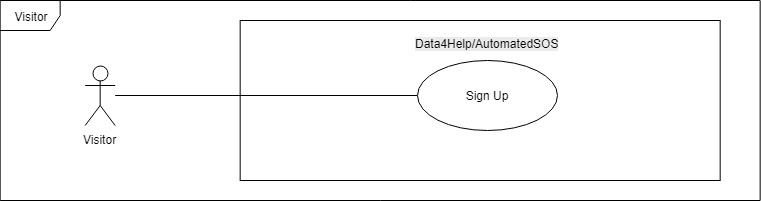
\includegraphics[width = 300pt]{images/Use-case/UCVisitor.jpg}
    \caption{Use case-Visitor.}
\end{figure}


\begin{center}
\begin{tabular}{|l|  p{8cm}|} \hline
    Name & {Sign Up} \\ \hline
    Actor & {Visitor} \\ \hline
    Entry Conditions & {The visitor has installed the application on his/her device.} \\ \hline
    Event Flows & {
        1. Click on the \say{Sign up} button.\newline
        2. Complete the mandatory fields providing the necessary informations. \newline
        3. Click on \say{Confirm} button. \newline
        4. The application checks that the provided data are complete and correct and saves them in the system.} \\ \hline
    Exit Conditions & {The user has completed the registration and can proceed to use the functionalities of the system.} \\ \hline
    Exceptions & {
        - The user is already registered.\newline
        - The information provided by the user are not complete/correct.\newline
        - The username is already taken. \newline
        The exceptions are handled by notifying the user and taking him back to the sign up activity.} \\ \hline
\end{tabular}
\end{center}

\begin{figure}[ht]
    \renewcommand{\thefigure}{\alph{figure}}
    \centering
    \captionsetup{labelformat=parens, labelsep=space, name=}
    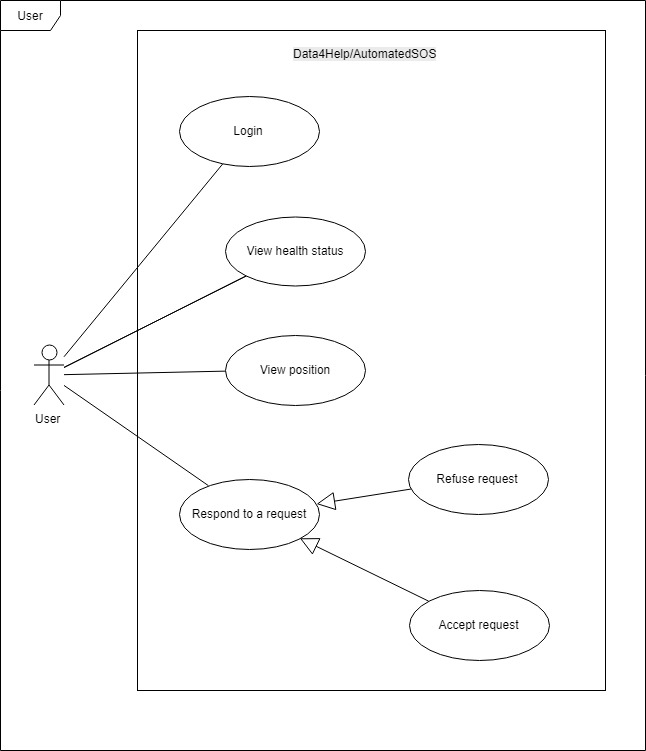
\includegraphics[width = 290pt]{images/Use-case/UCUser.jpg}
    \caption{Use case-User.}
\end{figure}

\begin{center}
\begin{tabular}{|>{\bfseries} l |  p{8cm} |} \hline
    Name & {Log-in} \\ \hline
    Actor & {User} \\ \hline
    Entry Conditions & {The user is successfully signed up.} \\ \hline
    Event Flows & {
    -The user opens the application on his/her device. \newline
    -The user inserts his/her credentials(username and password) in the apposite fields on the start page of Data4Help app. \newline
    -The user clicks on the \say{Log-in} button.} \\ \hline
    Exit Conditions & {The user is redirected to the view page of his/her position and his/her health parameters.} \\ \hline
    Exceptions & {
    -The user inserts a wrong username.\newline
    -The user inserts a wrong password.\newline
    All the exceptions are handled by showing a notification on the user's screen and taking him/her back to the log-in activity.} \\ \hline
\end{tabular}
\end{center}

\begin{center}
\begin{tabular}{|>{\bfseries} l |  p{8cm} |} \hline
    Name & {View health status} \\ \hline
    Actor & {User} \\ \hline
    Entry Conditions & {
    -The user is successfully logged in and he/she is on the Data4Help home-page.} \\ \hline
    Event Flows & {
    -The user clicks on the button \say{activities} and a list of the possible activities appears on the user's screen. \newline
    -The user choose the activity \say{view health status} from the list.} \\ \hline
    Exit Conditions & {The user is redirected to the view page in which he can observe his/her health parameters.} \\ \hline
    Exceptions & {
    -No parameters are available. \newline
    The exception is handled by showing a notification on the user's screen and he/she is redirected to the list of the possible activities.} \\ \hline
\end{tabular}
\end{center}

\begin{center}
\begin{tabular}{|>{\bfseries} l |  p{8cm} |} \hline
    Name & {View position} \\ \hline
    Actor & {User} \\ \hline
    Entry Conditions & {
    -The user is successfully logged in and he/she is on the Data4Help home-page.} \\ \hline
    Event Flows & {
    -The user clicks on the button \say{activities} and a list of the possible activities appears on the user's screen. \newline
    -The user choose the activity \say{view position} from the list.} \\ \hline
    Exit Conditions & {The user is redirected to the view page in which he/she can observe his/her position on a maps or by coordinates.} \\ \hline
    Exceptions & {
    -The position is not available. \newline
    The exception is handled by showing a notification on the user's screen and he/she is redirected to the list of the possible activities.} \\ \hline
\end{tabular}
\end{center}

\begin{center}
\begin{tabular}{|>{\bfseries} l | p{8cm} |} \hline
    Name & {Accept/refuse a request for personal data} \\ \hline
    Actor & {User} \\ \hline
    Entry Conditions & {
    -The user is successfully logged in.\newline
    -A third party sends a request to the user to access to his/her personal data.} \\ \hline
    Event Flows & {
    -A notification appears on the user's screen.\newline
    -The user clicks on the \say{accept} or on the \say{refuse} button.} \\ \hline
    Exit Conditions & {The user is redirected to the page he/she was surfing at the moment that the notification arrived.} \\ \hline
    Exceptions & {No possible exceptions.} \\ \hline
\end{tabular}
\end{center}

\begin{figure}[ht]
    \renewcommand{\thefigure}{\alph{figure}}
    \centering
    \captionsetup{labelformat=parens, labelsep=space, name=}
    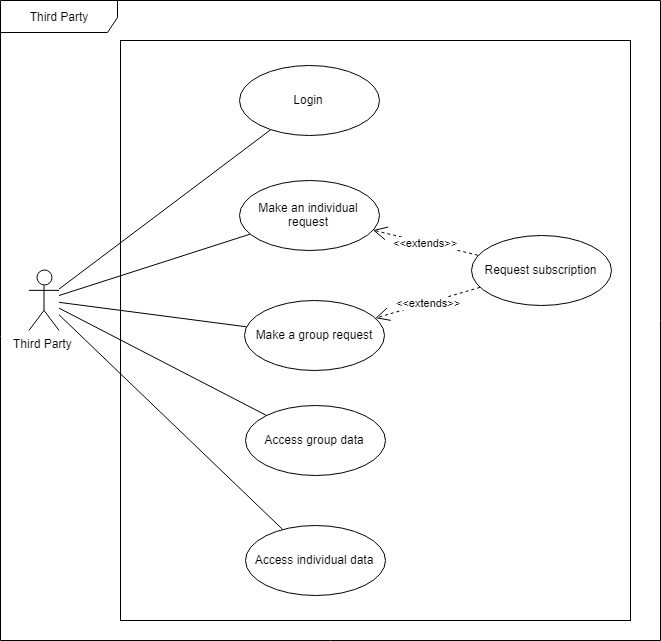
\includegraphics[width = 290pt]{images/Use-case/UCThirdParty.jpg}
    \caption{Use case-Third Party.}
\end{figure}

\begin{center}
\begin{tabular}{|>{\bfseries} l |  p{8cm} |} \hline
    Name & {Log-in} \\ \hline
    Actor & {Third Party} \\ \hline
    Entry Conditions & {The user is successfully signed up.} \\ \hline
    Event Flows & {
    -The third party opens the application on his/her device or he/she opens the Data4Help web-page. \newline
    -The third party inserts his/her credentials (username and password) in the apposite fields on the start page of Data4Help app or on the web-page. \newline
    -The third party clicks on the \say{Log-in} button.} \\ \hline
    Exit Conditions & {The third party is redirected to the home page of the Data4Help app or web-page} \\ \hline
    Exceptions & {
    -The third party inserts a wrong username.\newline
    -The third party inserts a wrong password.\newline
    All the exceptions are handled by showing a notification on the third party's screen and taking him/her back to the log-in activity.} \\ \hline
\end{tabular}
\end{center}

\begin{center}
\begin{tabular}{|>{\bfseries} l |  p{8cm} |} \hline
    Name & {Send a request for group of anonymized data} \\ \hline
    Actor & {Third party} \\ \hline
    Entry Conditions & {
    The third party is successfully logged in and it is on the home page of Data4Help web-site.} \\ \hline
    Event Flows & {
    -The third party clicks on the button \say{Create a group request}. \newline
    -The third party customizes some of the searching criteria. \newline
    -The third party clicks on the \say{send} button.} \\ \hline
    Exit Conditions & {A notification showing the outcome of the operation appears on the third party's screen and he/she is redirected to the home page of the Data4Help web-site.} \\ \hline
    Exceptions & {
    -No searching criteria are selected by the third party. \newline
    -Conflicting criteria are selected by the third party. \newline
    -The searching criteria corresponds to less than 1000 people.
    All the exceptions are handled by showing a notification on the third party's screen and taking him/her back to the home page of the Data4Help web-site.} \\ \hline
\end{tabular}
\end{center}

\begin{center}
\begin{tabular}{|>{\bfseries} l |  p{8cm} |} \hline
    Name & {Access to group of data} \\ \hline
    Actor & {Third party} \\ \hline
    Entry Conditions & {
    -The third party is successfully logged in and he/she is on the Data4Help home-page of the mobile application or on the web-site.} \\ \hline
    Event Flows & {
    -The third party clicks on the button \say{activities} and a list of the possible activities appears on the third party's screen. \newline
    -The third party chooses the activity \say{access to a group of data} from the list. \newline
    -A list of all the available group of data is shown on the third party's screen. \newline
    -The third party chooses a group of data he/she wants to access.} \\ \hline
    Exit Conditions & {The third party is redirected to the view page in which he can observe all the data available of that group.} \\ \hline
    Exceptions & {
    -No group of data are available. \newline
    -No data for the selected group are available. \newline
    The exception is handled by showing a notification on the third party's screen and he/she is redirected to the list of the possible activities.} \\ \hline
\end{tabular}
\end{center}

\begin{center}
\begin{tabular}{|>{\bfseries} l |  p{8cm} |} \hline
    Name & {Send a request for individual data} \\ \hline
    Actor & {Third party} \\ \hline
    Entry Conditions & {
    The third party is successfully logged in and it is on the home page of Data4Help mobile application or on the web-site.} \\ \hline
    Event Flows & {
    -The third party clicks on the button \say{Create an individual request}. \newline
    -The third party filles the following mandatory fields: Name, Surname, Fiscal Code or SSN. \newline
    -The third party clicks on the \say{send} button.} \\ \hline
    Exit Conditions & {A notification showing the outcome of the operation appears on the third party's screen and he/she is redirected to the home page of the Data4Help web-site. When the user accepts or refuse the request, a notification will appear on the third party's screen.} \\ \hline
    Exceptions & {
    -none is selected by the third party. \newline
    -an unexisting Fiscal Code or SSN is inserted by the third party. \newline
    -a wrong Fiscal Code or SSN is inserted by the third party. \newline
    All the exceptions are handled by showing a notification on the third party's screen and taking him/her back to the home page of the Data4Help web-site.} \\ \hline
\end{tabular}
\end{center}

\begin{center}
\begin{tabular}{|>{\bfseries} l |  p{8cm} |} \hline
    Name & {Access to individual data} \\ \hline
    Actor & {Third party} \\ \hline
    Entry Conditions & {
    -The third party is successfully logged in and he/she is on the Data4Help home-page of the mobile application or on the web-site.} \\ \hline
    Event Flows & {
    -The third party clicks on the button \say{Activities} and a list of the possible activities appears on the third party's screen. \newline
    -The third party chooses the activity "access to individual data" from the list. \newline
    -A list of all the individual's data to which the third party is authorized to access, is shown on the third his/her screen. \newline
    -The third party selects a user among the available data.} \\ \hline
    Exit Conditions & {The third party is redirected to the view page in which he can observe all the data available of that user.} \\ \hline
    Exceptions & {
    -No individual data are available. \newline
    -No data for the selected user are available. \newline
    The exception is handled by showing a notification on the third party's screen and he/she is redirected to the list of the possible activities.} \\ \hline
\end{tabular}
\end{center}

\begin{center}
\begin{tabular}{|>{\bfseries} l |  p{8cm} |} \hline
    Name & {Request Subscription to Data} \\ \hline
    Actor & {Third party} \\ \hline
    Entry Conditions & {
    -The third party is successfully logged in and he/she is in the process of making a request for group or individual data.} \\ \hline
    Event Flows & {
    -After filling the request procedure with the required criteria, the third party can click on the button "Request Subscription" to receive updated data as soon as they are created.  \newline
    -The request is sent to the system.} \\ \hline
    Exit Conditions & {A notification showing the outcome of the operation appears  on  the  third  party’s  screen  and  he/she  is redirected to the home page of the Data4Help web-site.} \\ \hline
    Exceptions & {
    -This use case is an extension of the \say{Data Request} use cases and inherits all its parent's exceptions. } \\ \hline
\end{tabular}
\end{center}

\begin{figure}[ht]
    \renewcommand{\thefigure}{\alph{figure}}
    \centering
    \captionsetup{labelformat=parens, labelsep=space, name=}
    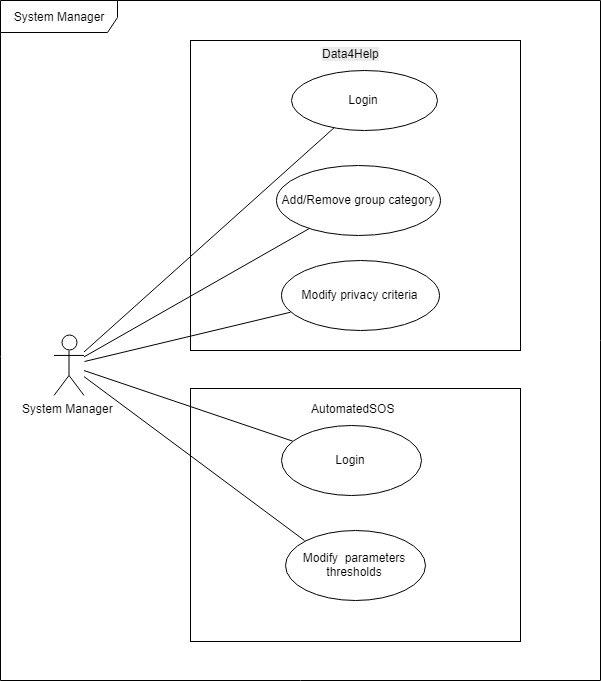
\includegraphics[width = 290pt]{images/Use-case/UCSystemManager.jpg}
    \caption{Use case-System Manager.}
\end{figure}

\begin{center}
\begin{tabular}{|>{\bfseries} l |  p{8cm} |} \hline
    Name & {Login} \\ \hline
    Actor & {System Manager} \\ \hline
    Entry Conditions & {
    -No entry conditions.} \\ \hline
    Event Flows & {
    -The system manager access Data4Help or AutomatedSOS back-end system on his/her device.  \newline
    -The system manager inserts his/her credentials (username  and  password)  in  the  apposite  fields  of the back-end system.} \\ \hline
    Exit Conditions & {The third party is redirected to the control panel of the back-end system.} \\ \hline
    Exceptions & {
    -The system manager inserts a wrong username. \newline
    -The system manager inserts a wrong password. \newline
    All the exceptions are handled by showing a notification on the system manager's screen and taking him/her back to the log-in activity. } \\ \hline
\end{tabular}
\end{center}

\begin{center}
\begin{tabular}{|>{\bfseries} l |  p{8cm} |} \hline
    Name & {Add/Remove Group Category} \\ \hline
    Actor & {System Manager} \\ \hline
    Entry Conditions & {
    The system manager is logged in Data4Help back-end system successfully.} \\ \hline
    Event Flows & {
    -The system manager updates Data4Help architecture adding or removing a group category.} \\ \hline
    Exit Conditions & {The system manager is redirected to the control panel of the back-end system.} \\ \hline
    Exceptions & {
    No exceptions.} \\ \hline
\end{tabular}
\end{center}

\begin{center}
\begin{tabular}{|>{\bfseries} l |  p{8cm} |} \hline
    Name & {Modify Privacy Criteria} \\ \hline
    Actor & {System Manager} \\ \hline
    Entry Conditions & {
    The system manager is logged in Data4Help back-end system successfully.} \\ \hline
    Event Flows & {-The system manager updates Data4Help architecture modifying the privacy criteria.} \\ \hline
    Exit Conditions & {The system manager is redirected to the control panel of the back-end system.} \\ \hline
    Exceptions & {
    No exceptions.} \\ \hline
\end{tabular}
\end{center}

\begin{center}
\begin{tabular}{|>{\bfseries} l |  p{8cm} |} \hline
    Name & {Modify Health Parameters Thresholds} \\ \hline
    Actor & {System Manager} \\ \hline
    Entry Conditions & {
    The system manager is successfully logged in AutomatedSOS back-end system.} \\ \hline
    Event Flows & {
    -The system manager updates the database containing the health parameters thresholds.} \\ \hline
    Exit Conditions & {The system manager is redirected to the control panel of the back-end system.} \\ \hline
    Exceptions & {
    No exceptions.} \\ \hline
\end{tabular}
\end{center}
\clearpage


\section{Sequence Diagrams}
\begin{figure}[H]
    \setcounter{figure}{0}
    \renewcommand{\thefigure}{\alph{figure}}
    \makebox[\textwidth]{
        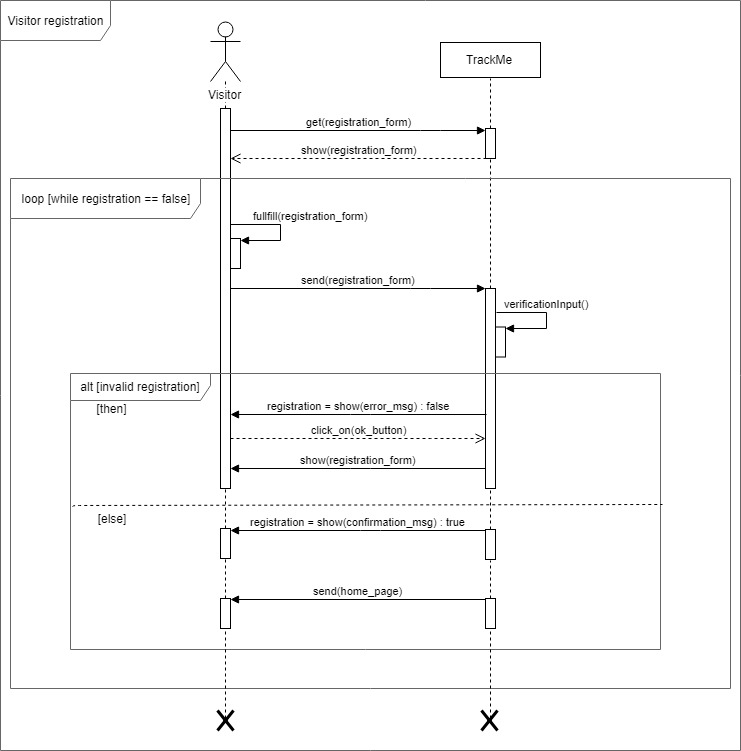
\includegraphics[width=1.4\linewidth]{images/Sequence-diagram/SDVisitor_registration.jpg}
    }
    \captionsetup{labelformat=parens, labelsep=space, name=}
    \caption{Visitor registration.}
\end{figure}

\begin{figure}[H]
    \renewcommand{\thefigure}{\alph{figure}}
    \makebox[\textwidth]{
        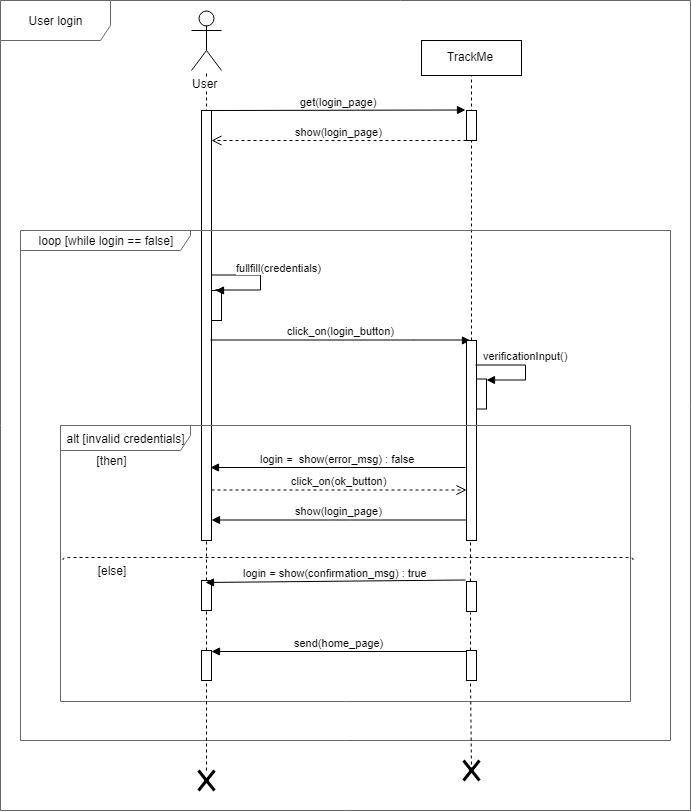
\includegraphics[width=1.3\linewidth]{images/Sequence-diagram/SDUser_login.jpg}
    }
    \captionsetup{labelformat=parens, labelsep=space, name=}
    \caption{User login.}
\end{figure}

\begin{figure}[H]
    \renewcommand{\thefigure}{\alph{figure}}
    \makebox[\textwidth]{
        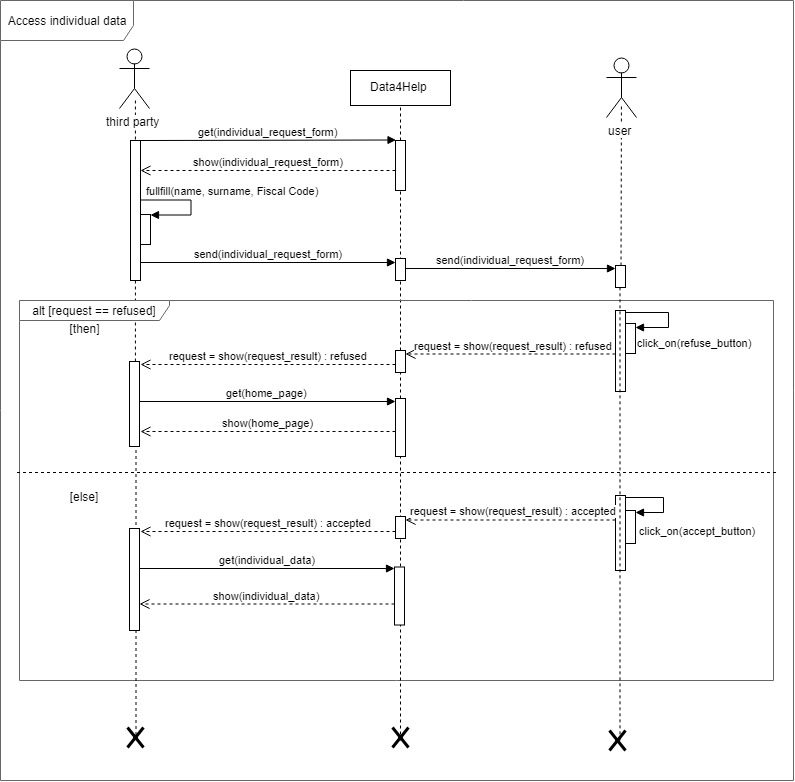
\includegraphics[width=1.4\linewidth]{images/Sequence-diagram/SDAccess_to_ind_data.jpg}
    }
    \caption{Third party accesses to the data of a single user.}
\end{figure}

\begin{figure}[H]
    \renewcommand{\thefigure}{\alph{figure}}
    \makebox[\textwidth]{
        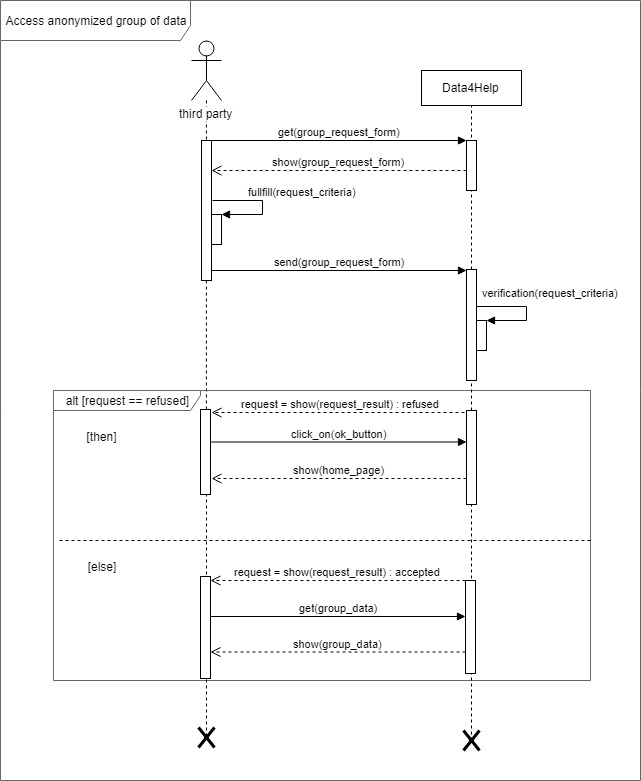
\includegraphics[width=1.25\linewidth]{images/Sequence-diagram/SDAccess_group_data.jpg}
    }
    \caption{Third party accesses to a group of anonymized data.}
\end{figure}

\begin{figure}[H]
    \renewcommand{\thefigure}{\alph{figure}}
    \makebox[\textwidth]{
        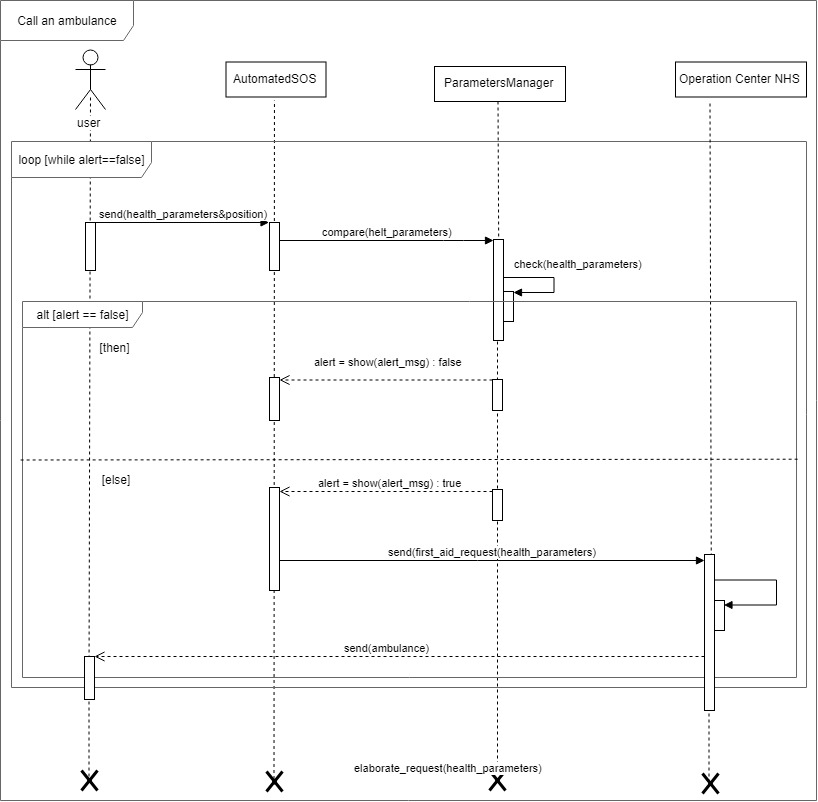
\includegraphics[width=1.4\linewidth]{images/Sequence-diagram/SDAutomatedSOS.jpg}
    }
    \caption{AutomatedSOS sends an ambulance.}
\end{figure}

\clearpage

\section{Performance Requirements}
The system has to be able to respond to a huge number of transactions simultaneously. The service should be able to scale depending on the number of active users. 
Speed and performance are critical especially for AutomatedSOS service, since it must guarantee to contact the Operations Center within 5 seconds from the time an anomaly is detected.

\section{Design Constraints}
\subsection{Standards compliance}
    \begin{itemize}
        \item Health parameters are stored according the international units of measure.
        \item Position is stored according geographic coordinates system.
        \item SSN or Fiscal Code format changes according to the country of usage.
    \end{itemize}

\subsection{Hardware limitations}
\begin{itemize}
\item Mobile App
    \begin{itemize}
        \item Apple or Android smartphone
        \item Apple, Android, Fitbit or Garmin wearables
        \item 3G/4G/WiFi connection
        \item Bluetooth
        \item GPS
        \item Heart rate, temperature, blood glucose level, accelerometer sensors
    \end{itemize}
\item Web App
    \begin{itemize}
        \item Devices that supports modern browsers such as Google Chrome, Mozilla Firefox, Microsoft Edge, Apple Safari, etc.
    \end{itemize}
\end{itemize}
\subsection{Any other constraint}

\subsubsection{Regulatory Policies}
The system will be subject to the privacy requirements enforced by the national law. In order to respect the minimum constraints, the system will ask for users' permission to store their data and to let third parties access to their personal informations.

\subsubsection{Interfaces}
    Sensors interact with Data4Help through an apposite API (healthKit for iOS\cite{healthKit}, Sensors API for Android\cite{sensorsAPI}).
    AutomatedSOS interacts with the Operations Center through an interface provided by the NHS or trough a VoIP API.
    Data4Help uses Google Maps API to show the position of a user on a mobile or web app.
    Google Maps API is also used to transform a position on a map into an address while composing a group request.

\subsubsection{Level of Criticality}
Since an unexpected fault in Data4Help acquisition could implies very important consequences on the safeness of AutomatedSOS users, it is critical that the system is almost always available.

\subsubsection {Parallel operations}
The system has to support multiple concurrent requests. Individual data may be accessed concurrently by more than one third party. Also Data4Help will be able to record data from many different users at the same time.

\section{Software System Attributes}
\subsection{Reliability}
The system should offer a level of reliability such that core functions crash-down occur rarely and can promptly be restored.
The application should aim to a 24/7 reliability, of course small variations from the ideal case are tolerable. 

\subsection{Availability}
The system is required to have an availability of 99.99\%, meaning that the maximum downtime accepted every year is of 1 hour. To ensure this requirement the system will have to be implemented with redundancy of data in order to overcome potential malfunctioning.

\subsection{Security}
It is important to ensure that the system is adequately protected against attacks to ensure the privacy and the safety of the users.
The system must guarantee that only authorized third parties are able to access individuals data and that only the system managers can update the internal functionalities.
All the users' data should be encrypted both during the client-server communication and on the server database.
The data center should also be protected against natural disasters such as fire or floods. 

\subsection{Maintainability}
The system should be easy to maintain and update. Services such as Data4Help and AutomatedSOS could need in the future some improvement in their functionalities (such as the addiction of a new revolutionary sensor for Data4Help or the changes in the thresholds in AutomatesSOS), so it's crucial that they are designed in a flexible way.
In order to observe this constraint, the system will be implemented following the most common software engineering best practices and will be detailed with a complete and specific documentation.

\subsection{Portability}
To ensure the portability of the core service, the database and the back-end system will be implemented avoiding platform dependent programming languages.
Also the web client applications will be designed following the W3C standards, in order to ensure a correct rendering of the page in all major browsers.